\chapter{Simulation}

The frontend can be quite interesting as just a way to survey a city from a bird's eye view. The program's real use lies in data analysis, though, as the task description suggests. Over the semester, I tried multiple approaches for creating an agent-based simulation, with all but the last attempt failing due to technical circumstances.

\section{Deprecated versions}

The first concept was very simple. Each agent would pick a random building to start at and head to in a straight line, with a constant speed. Each agent would be shown in the graphical scene, and the visuals would not be unlike an ant colony. The backend simulated movement in one minute steps, and after each one, the modified agents would be collected and sent over the websocket in a few chunks, so as to reduce the chances of the socket crashing. The problem here was one of scalability. Fifty or a hundred agents could easily be processed and shown in real time, but that obviously was not enough to draw any meaningful conclusions about transit behaviour. Displaying more agents caused a simply unacceptable framerate of three frames per second at most. Although I used the same model for every agent, batching and caching could not be used due to the chaotic nature of their overall movement.
\begin{figure}[h]
    \centering
    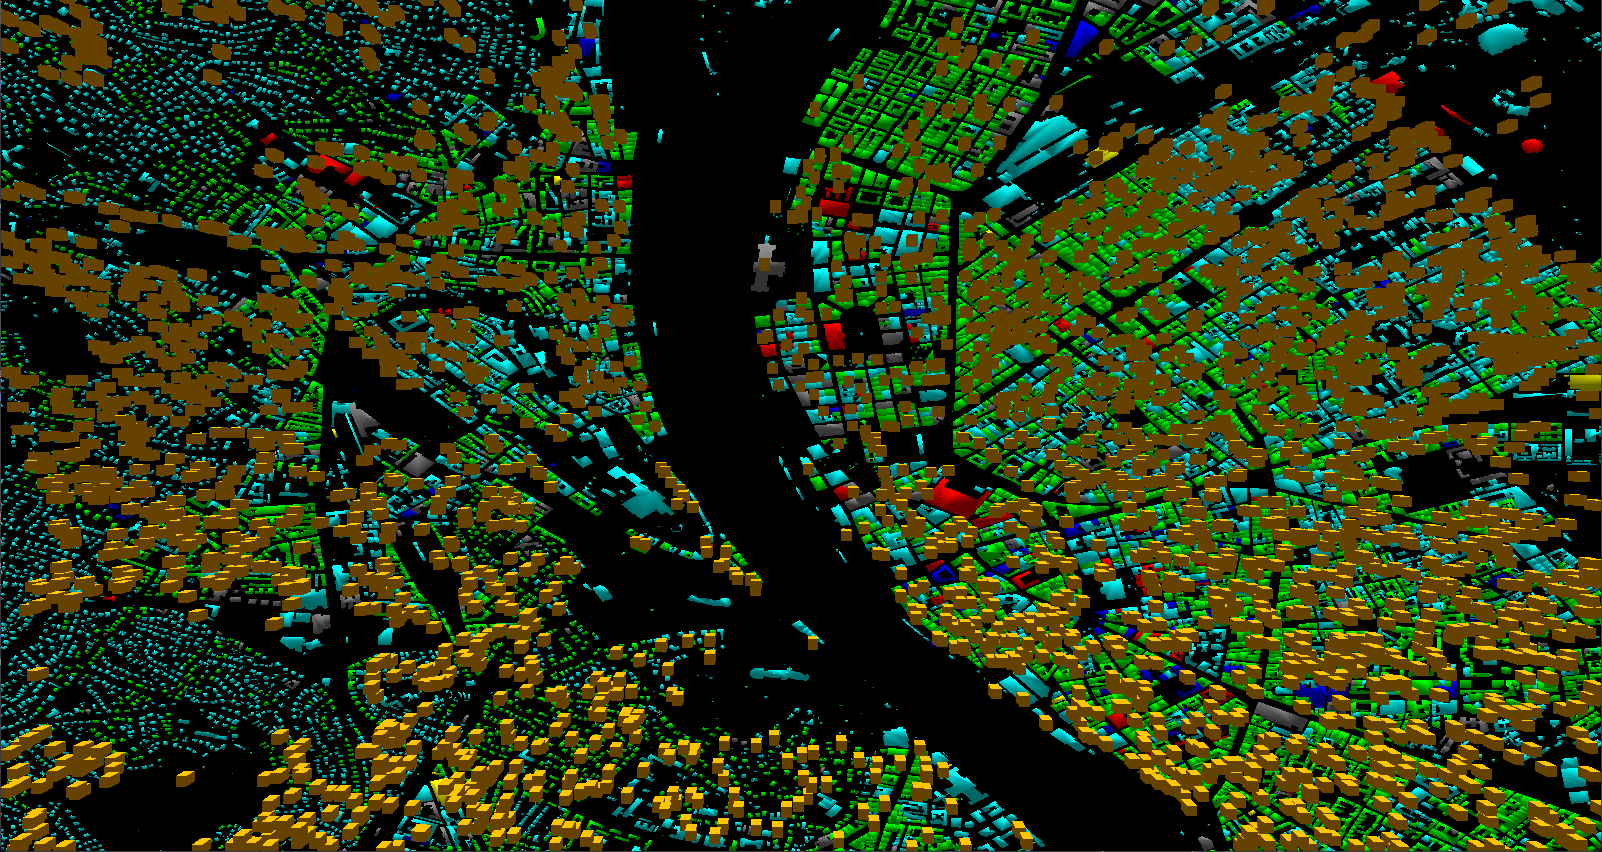
\includegraphics[width=140mm, keepaspectratio]{images/overlay_v1.png}
    \caption{An array of cubes displayed over the city of Budapest, each representing an agent\ \label{overlay_v2}}
\end{figure}

The second version improved performance by processing the agent updates non-visually and dividing up the playfield into relatively small chunks to act as a heatmap; it was a separately renderable on top of the main scene. Each update's coordinates were fed into the overlay, and an opacity value was calculated for every chunk. The result was a serviceable tool that, while updating constantly, still had bad performance. A new object cache was being created every time I opened the heatmap UI, and this taxed the rendering thread heavily. However, once all updates have been processed, the performance was decent. This gave me the idea of running full simulations as fast as possible, and only transferring a minimal amount of information over the socket.
\begin{figure}[h]
    \centering
    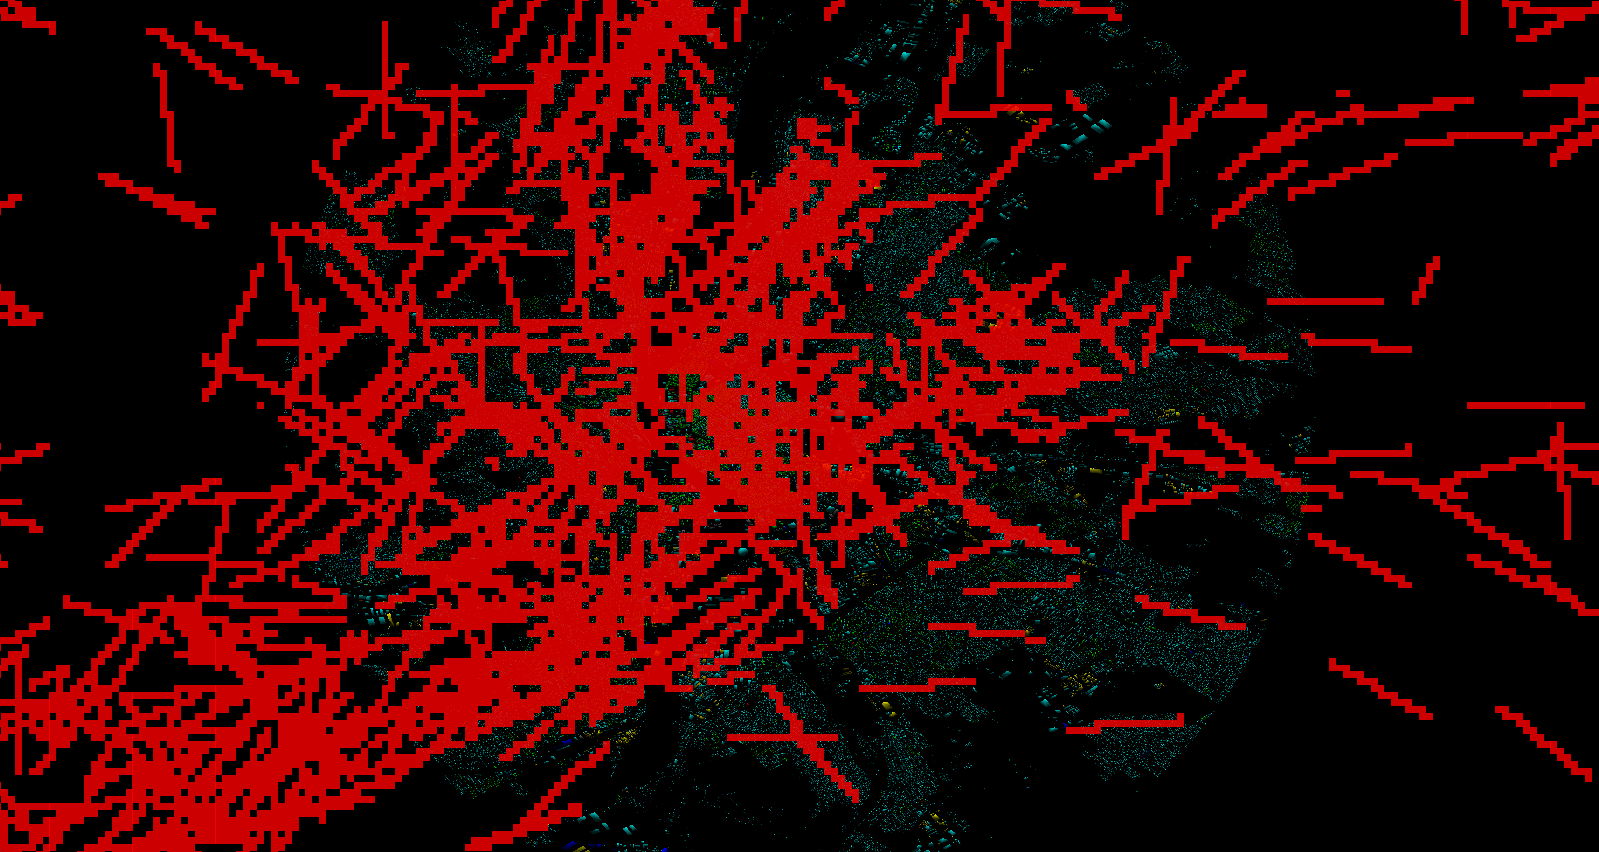
\includegraphics[width=140mm, keepaspectratio]{images/overlay_v2.png}
    \caption{An overlay with flattened opacity, displayed over the city of Budapest. Agent paths are randomised and are traversed in a straight line\ \label{overlay_v2}}
\end{figure}

\section{The working implementation}

I ended up keeping the agent idea, but highlighted the need for the frontend to be uninvolved aside from requesting and displaying content. As a first step, the map needs to be loaded -- as well as the building data, the backend sends over a baseline coordinate pair that can be used as the origin of the graphics scene. This is important as the server should not and can not have any knowledge of the display it's sending data to. As such, the heatmap's chunk size is scaled to real world coordinates and converted back after the response. The client can choose all parameters of the simulation, set with the user's settings.
\begin{figure}[h]
    \centering
    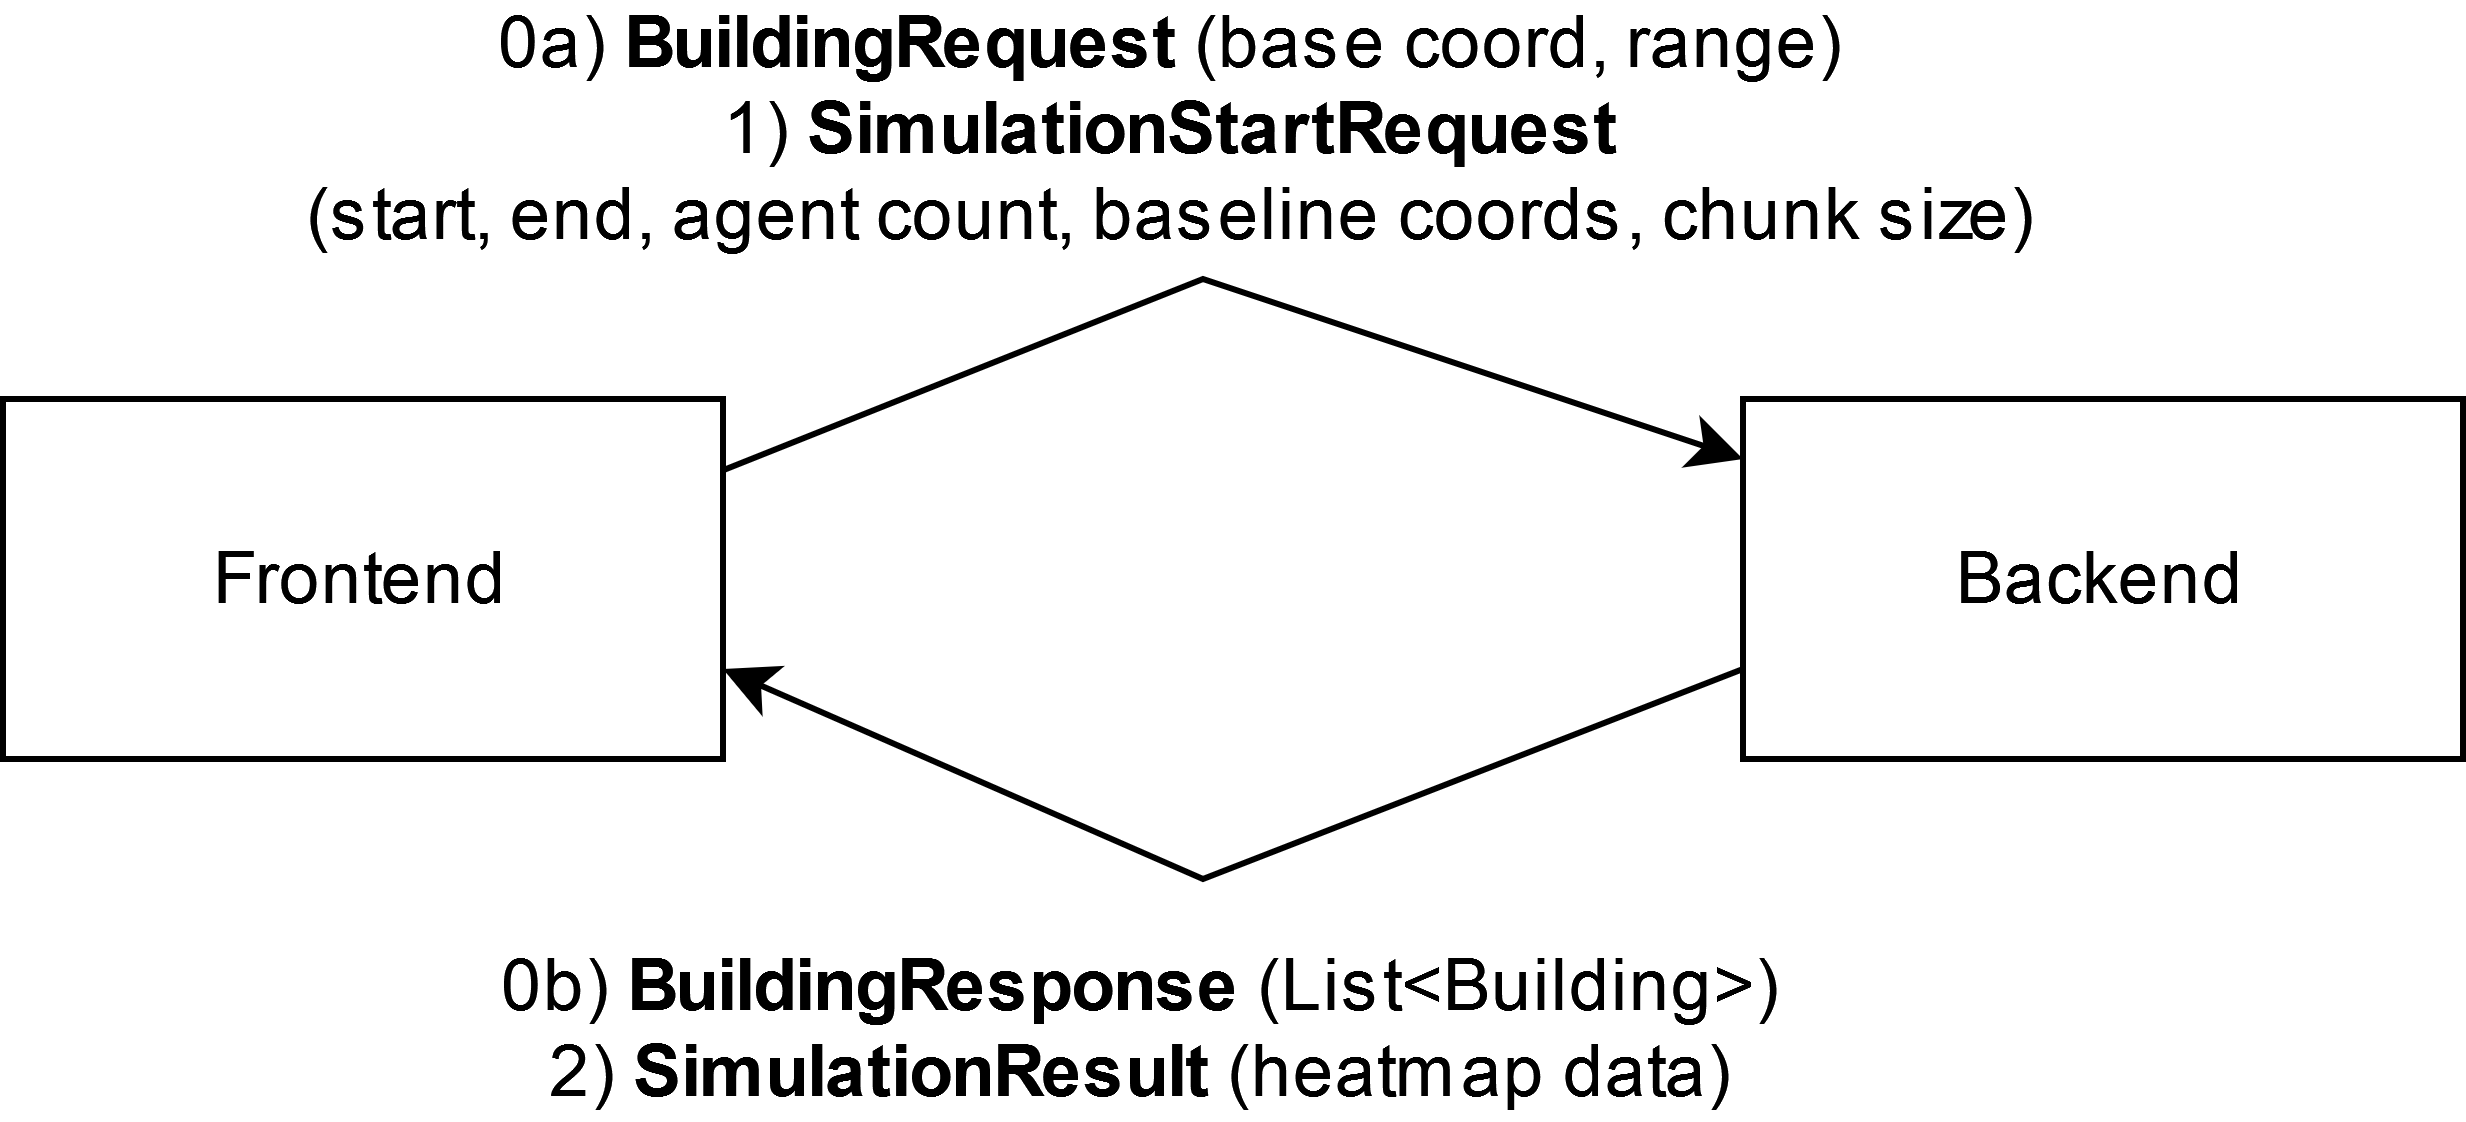
\includegraphics[width=100mm, keepaspectratio]{images/simu_network.png}
    \caption{An overview of the network communication required for a simulation\ \label{simu_network}}
\end{figure}

The server starts each simulation from scratch. The requested amount of agents is randomly distributed on the map, with the buildings chosen from the database, weighted by the "capacity" column: a large residential building is more likely to have agents start there than a small boutique. Each person can then choose a target building every minute, but may also choose to remain where they are. With a resolution of one second, the difference between the goal and the current location is determined, normalised, and the agent is nudged along by adding this value to its position, multiplied by the agent's speed. As of now, the speed is pre-determined in the Agent class, helping the setup of different vehicle types in the future.

The simulation constantly updates an instance of the HeatmapData class, adding one to the value of the cell that contains the current step. The grid size is received in degrees of latitude/longitude. The correct cell's id is calculated by flooring the coordinates using the baseline and grid size. The map is not pre-allocated, the desired cell is created on the fly if it does not exist -- this reduces data transfer significantly. Updates are grouped by minute and then by agent. Once the final state is reached, a SimulationResult message is sent back with the heatmap cells.

The data is transformed by the client, scaling the coordinates contained in each cell's identifier back, and placing each integer into the correct slot of the libGDX heatmap. Every value is absolute, scaling is done at render time.

\subsection{Building selection logic}

People in the simulation choose targets based on a simplified statistical model. They may be in one of four primary age groups: children, teens, adults or the elderly. Time of day, age group and building type can be represented as a three-dimensional distribution. Some building types (such as schools) are visited rarely at night, but very often in mornings. Age group and building type is connected as well: children are generally not expected to travel to industrial complexes. 

I represented this as two static distributions, stored on the server's side. The chance of a given agent travelling to a certain building type is calculated by multiplying the time-type and age-type values together. The sum of all types for the given situation gives an absolute value that is expected to be around 100 at most. Using this, agents first decide whether they want to travel at all: the maximum chance is about 50\%. Then, the target type is picked at random, weighted by the calculated chances. If the calculated building variety is the same as the current building, the agent does not leave; otherwise, a random building is picked, with closer buildings being slightly more likely than far away ones.

The method thus has three variables calculated at random. This requires many more agents than a more sophisticated model, but its accuracy is acceptable, provided the required processing power is available. Since the model is based on individual decisions, future expansion is not too difficult -- more variables can be added as needed. Travel time is not taken in to account at all, making this version unsuitable for planning transit lines.